\chapter{Load Balancing}\label{chapter:load_balancing}
% Say it only uses number of elements, point to results for N influence on GPUs

A well made multi-block mesh can distribute the work evenly between the different worker processes
without needing runtime adjustment if the topology and areas of more expensive computation stay the
same during the whole computation. This is complicated by the fact that, as seen in
Chapter~\ref{chapter:adaptive_mesh_refinement}, the mesh elements can increase their polynomial
order and split into multiple smaller elements in areas where the solution accuracy is estimated to
be unsatisfactory. Unless the regions of interest happen to be evenly distributed between the
different processes, this will lead to an imbalance as some processes are left with more elements,
or higher-order elements, within their domain.

\begin{figure}[H]
	\centering
	\subfloat[Mesh before refining]
	{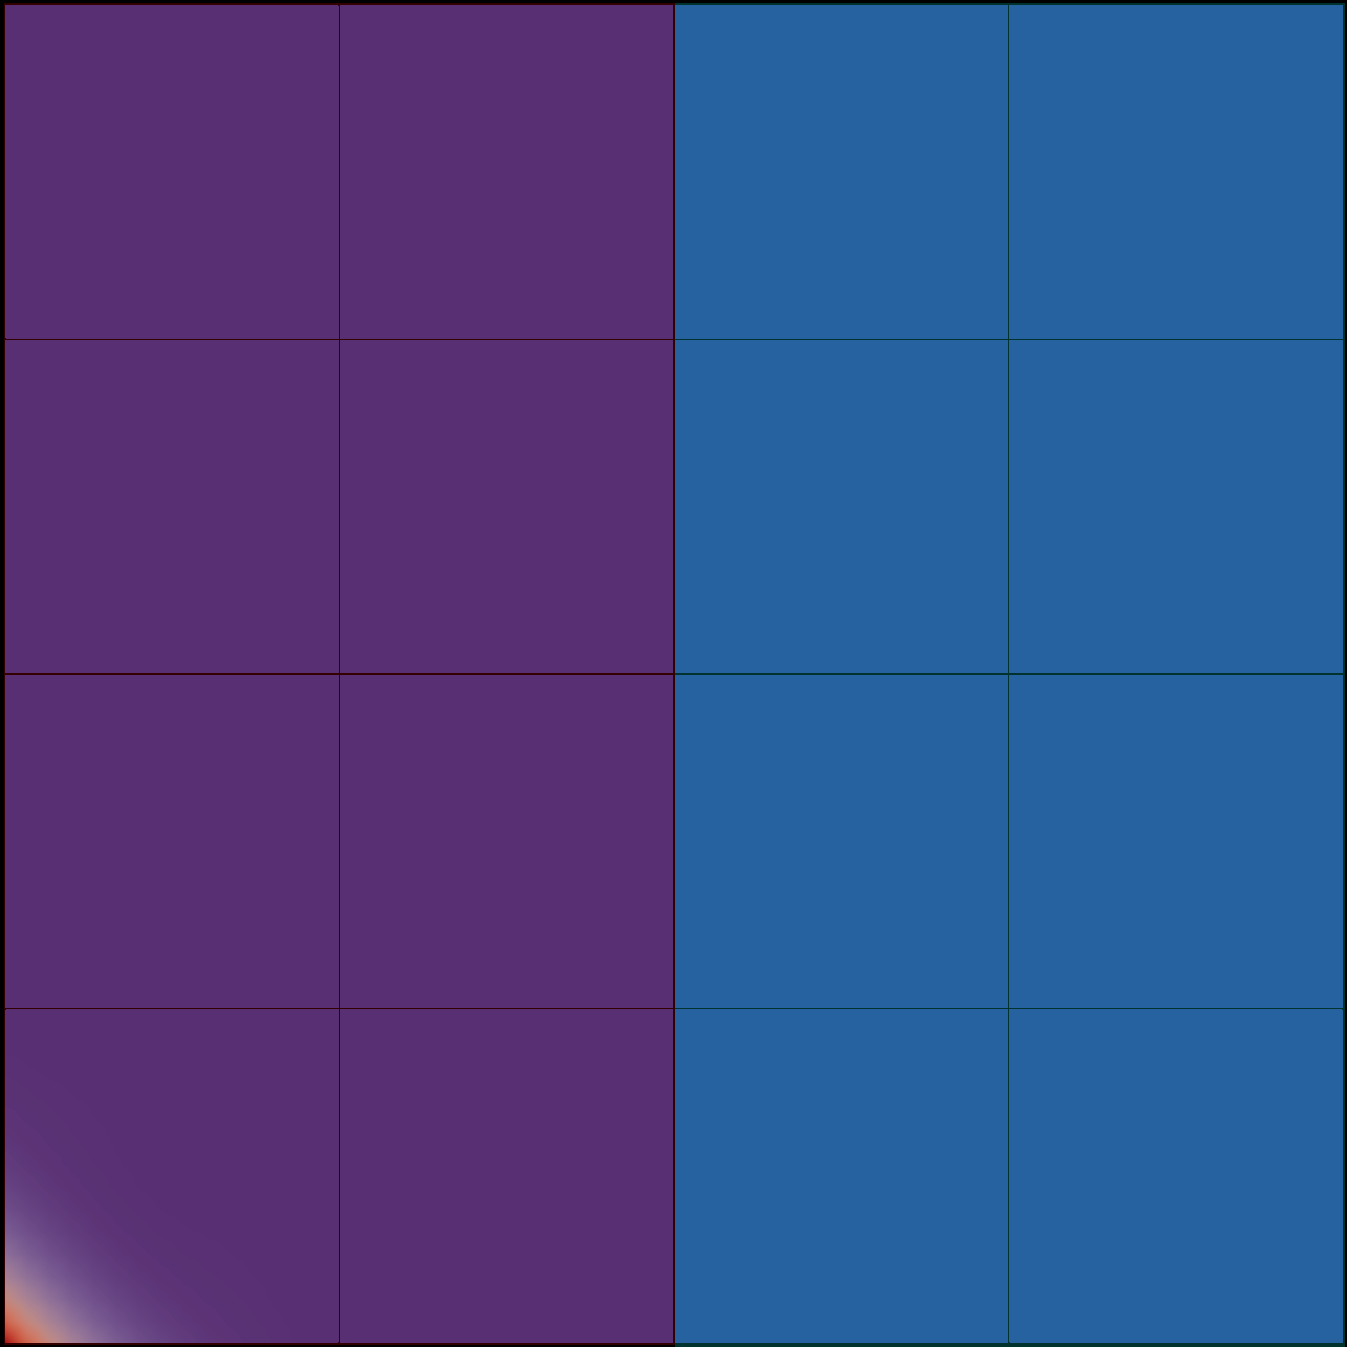
\includegraphics[width=0.45\textwidth]{Chapter_load_balancing/media/load_imbalance_initial}\label{fig:mesh_imbalance_initial_lb}}
	\hfill
	\subfloat[Mesh after refining]
	{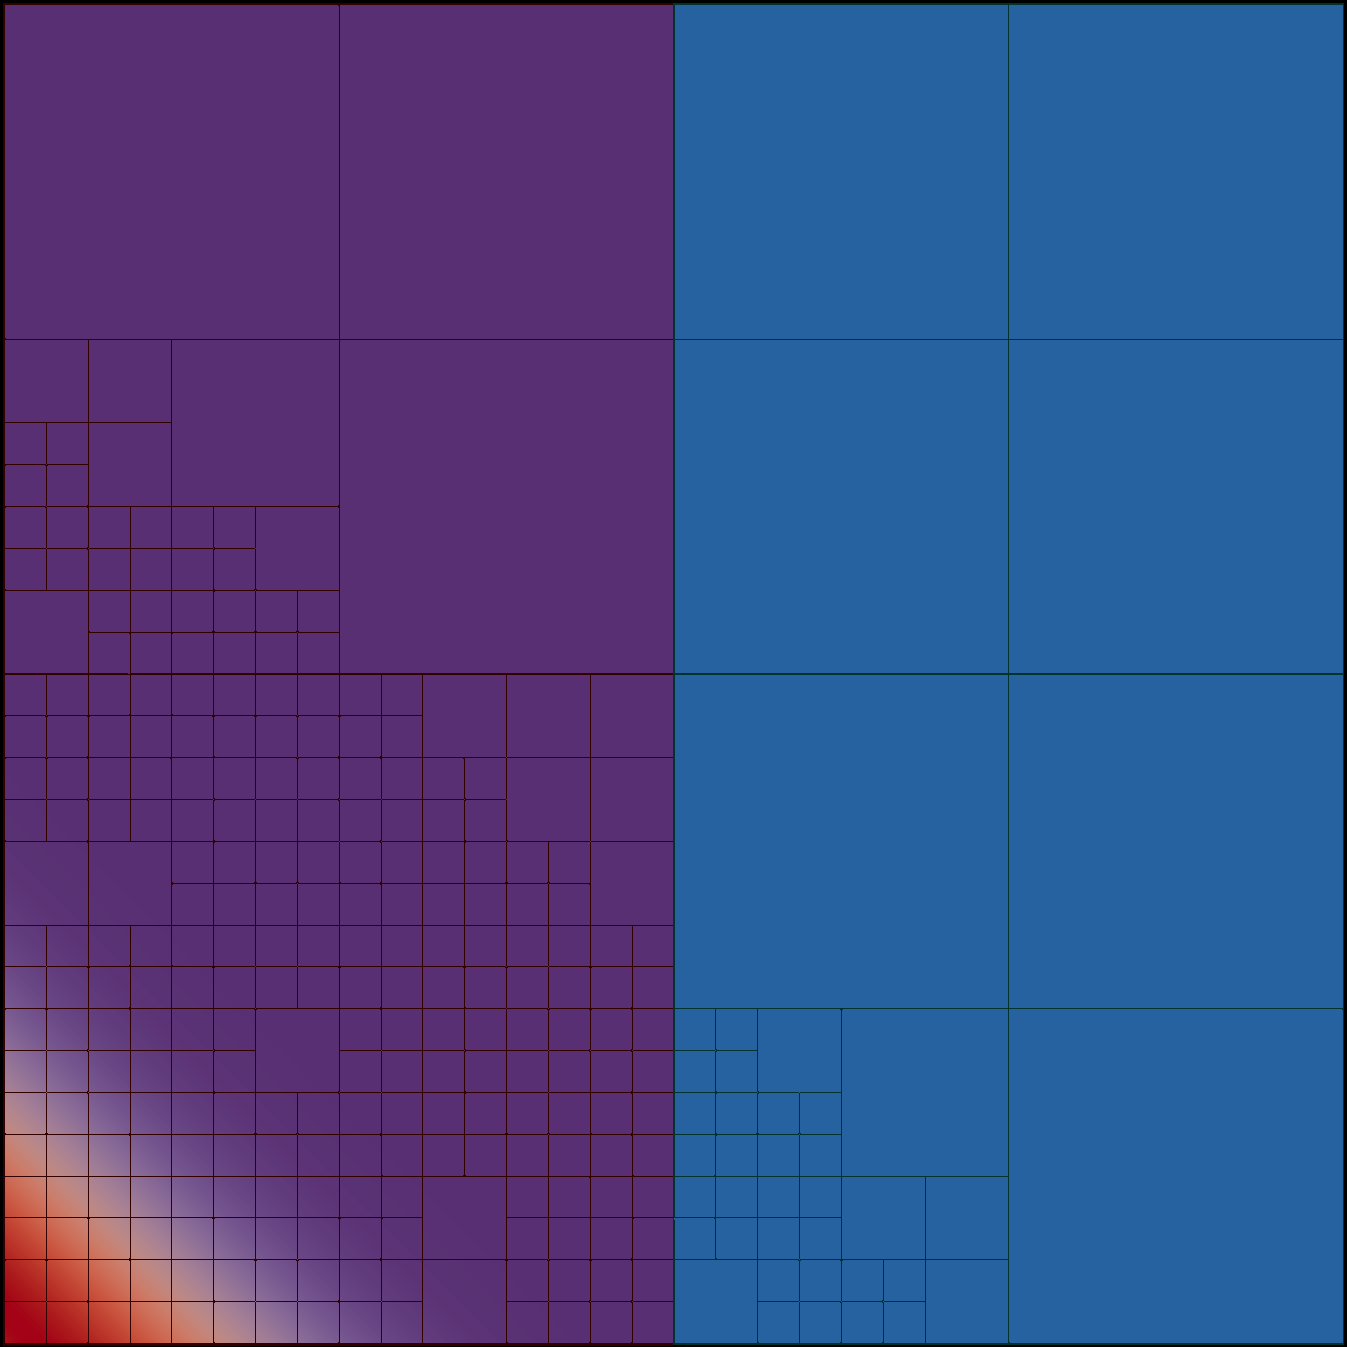
\includegraphics[width=0.45\textwidth]{Chapter_load_balancing/media/load_imbalance}\label{fig:mesh_imbalance_after_refinement_lb}}
	\caption{Load imbalance: The elements have split unequally in the two worker \acrshortpl{acr:GPU}, one having a higher computational load. (a) Before refining (b) After refining}\label{fig:load_imbalance_lb}
\end{figure}

The wall clock time of the simulation will be driven by the most heavily loaded process, as the
processes have to synchronise at each time step. The more lightly loaded processes will simply wait
for the other to finish computing.

In order to maintain good performance as the mesh is refined, we will need to perform dynamic load
balancing. Dynamic load balancing seeks to even out the computational load between the different
processes. The algorithm for load balancing needs to be fast, to be executed often and to keep the
mesh optimal for a longer period without overshadowing the solution time. The worker processes in
this work use \acrshortpl{acr:GPU} for their computations. Because transfers between
\acrshortpl{acr:GPU} are expensive, the algorithm needs to limit transfers both during the load
balancing process and during computation afterwards. The workers are made up of one
\acrshort{acr:CPU} core and one entire \acrshort{acr:GPU}. This means that the worker's processing
power is mostly generated by the \acrshort{acr:GPU}, and the algorithm needs to use it as much as
possible. The algorithm will need to have as many parts as possible running on the
\acrshort{acr:GPU}, in parallel. Finally, the algorithm needs to use as little additional
\acrshort{acr:GPU} memory as possible, as these processors have limited memory, especially compared
to \acrshortpl{acr:CPU}.

The algorithm needs to select which elements to send from one \acrshort{acr:GPU} to another. Many
such algorithms exist, notably graph-based algorithms~\cite{Karypis1998} and one-dimensional
algorithms~\cite{Pinar2004}, often called \textit{\acrfull{acr:CCP}}. \Acrlong{acr:CCP} will be used
here for its relative speed. This will require a scheme to transform our domain from two-dimensional
space to one-dimensional space, as required by the algorithm.

Here, the repartitioning scheme uses \textit{\acrfullpl{acr:SFC}}, more specifically the Hilbert
Curve. \Acrshortpl{acr:SFC} map multi-dimensional space to one-dimensional space. This space can be
partitioned in segments, and upon change of the size of these segments elements can then be sent or
received from the ends of these segments. In addition, these curves are fast to generate, use low
memory, and maximise locality. Elements that are close in curve space will also be close by in the
space used for computations. This limits the number of interfaces between processes.

\section{Hilbert Curve}\label{section:load_balancing:hilbert_curve}

The Hilbert curve, developed by D. Hilbert~\cite{Hilbert1891}, is a specific kind of space-filling
curve as described by G. Peano~\cite{Peano1890}. This curve works for 2D domains with equal and
power of two resolution in x and y. Some newer research~\cite{Haverkort2011} shows how such curves
can be expanded to three dimensions, and arbitrary domains.

\begin{figure}[H]
	\centering
	\subfloat[First level]
	{\includesvg[width=0.3\textwidth]{Chapter_load_balancing/media/hilbert_curve_K2}\label{fig:hilbert_k2}}
	\hfill
	\subfloat[Second level]
	{\includesvg[width=0.3\textwidth]{Chapter_load_balancing/media/hilbert_curve_K4}\label{fig:hilbert_k4}}
	\hfill
	\subfloat[Third level]
	{\includesvg[width=0.3\textwidth]{Chapter_load_balancing/media/hilbert_curve_K8}\label{fig:hilbert_k8}}
	\caption{Hilbert curve: The first thee Hilbert curves. (a) \(2\times2\) (b) \(4\times4\) (c) \(8\times8\)}\label{fig:hilbert_curves}
\end{figure}

Figure~\ref{fig:hilbert_curves} shows the first three levels of the Hilbert curve. The curve
successfully maps our 2D domain to a 1D one along the curve. That 1D domain can then be partitioned
between the different worker \acrshortpl{acr:GPU}. As illustrated in the figure, the elements have
good locality and no jumps exist. Wherever the curve is cut, elements on the resulting segments are
close together. This is the first desirable property of the curve for this program, as we aim to
reduce the contact area between the mesh blocks dispatched to each \acrshort{acr:GPU}. The iterative
nature of those curves is also apparent when put side by side. Each increasing level of the curve
follows the general path of the previous curve. Iteration is one of the possible ways to generate
this curve. It will be used to generate the initial meshes used by the program, as well as to
re-number elements when the mesh refines.

\subsection{Generation}\label{subsection:load_balancing:hilbert_curve:generation}

We choose a table-driven algorithm to generate meshes. Each element has one of four possible states
\(s\): \(s \in \left \{H, A, R, B \right \} \). This state determines the state and ordering of the
four children elements obtained when increasing the level of the curve. The four states and their
resulting children are shown in the following figure.

\begin{figure}[H]
	\centering
	\subfloat[H splitting: \newline \(A, H, H, B\)]
	{\includesvg[width=0.23\textwidth]{Chapter_load_balancing/media/hilbert_split_H}\label{fig:hilbert_split_H}}
	\hfill
	\subfloat[A splitting: \newline \(H, A, A, R\)]
	{\includesvg[width=0.23\textwidth]{Chapter_load_balancing/media/hilbert_split_A}\label{fig:hilbert_split_A}}
	\hfill
	\subfloat[R splitting: \newline \(B, R, R, A\)]
	{\includesvg[width=0.23\textwidth]{Chapter_load_balancing/media/hilbert_split_R}\label{fig:hilbert_split_R}}
	\hfill
	\subfloat[B splitting: \newline \(R, B, R, H\)]
	{\includesvg[width=0.23\textwidth]{Chapter_load_balancing/media/hilbert_split_B}\label{fig:hilbert_split_B}}
	\caption{The four states splitting, with their children's state and ordering.}\label{fig:hilbert_splits}
\end{figure}

When put together, and assigning \(H\) as the first state of the mesh, the mesh can be iteratively
constructed to the required level as shown in Figure~\ref{fig:hilbert_levels}.

\begin{figure}[H]
	\centering
	\subfloat[Level 0]
	{\includesvg[width=0.3\textwidth]{Chapter_load_balancing/media/hilbert_level_0}\label{fig:hilbert_l0}}
	\hfill
	\subfloat[Level 1]
	{\includesvg[width=0.3\textwidth]{Chapter_load_balancing/media/hilbert_level_1}\label{fig:hilbert_l1}}
	\hfill
	\subfloat[Level 2]
	{\includesvg[width=0.3\textwidth]{Chapter_load_balancing/media/hilbert_level_2}\label{fig:hilbert_l2}}
	\caption{First levels of the Hilbert curve with statuses \(s\) (\(s \in \left \{ H, A , B , R \right \} \)).}\label{fig:hilbert_levels}
\end{figure}

This construction can be summarised in Tables~\ref{table:children_state}
and~\ref{table:children_ordering}. The ordering of the children elements is from the bottom left
element, in counter-clockwise order. 

\begin{figure}[H]
	\centering
	\includesvg[width=0.3\textwidth]{Chapter_load_balancing/media/child_order}
	\caption{Children numbering: The \(j = 0, 1, 2, 3\) children of an element, used to assign states and ordering.}\label{fig:child_order}
\end{figure}

These tables are implemented directly in the code, with the state defined as an enumeration from 0
to 3 and the tables as arrays. The state indexes into the array to get the resulting ordering and
states. This gives the state \(S(s, j)\) of the j\textsuperscript{th} child element of a parent
element as a function of the state \(s\) of the parent element. The same goes for the ordering \(p\)
of the children, \(P(s, j)\).

\begin{table}[H]
	\begin{center}
		\begin{tabular}{ c | c c c c} 
			\(S\left ( s, j \right )\) & \(j = 0\) & \(j = 1\) & \(j = 2\) & \(j = 3\)  \\
			\hline
			\(s = H\) & \textcolor{vs_red}{\(A\)} & \textcolor{vs_red}{\(B\)} & \textcolor{vs_red}{\(H\)} & \textcolor{vs_red}{\(H\)} \\ 
			\(s = A\) & \textcolor{vs_blue}{\(H\)} & \textcolor{vs_blue}{\(A\)} & \textcolor{vs_blue}{\(A\)} & \textcolor{vs_blue}{\(R\)} \\
			\(s = R\) & \textcolor{vs_teal}{\(R\)} & \textcolor{vs_teal}{\(R\)} & \textcolor{vs_teal}{\(B\)} & \textcolor{vs_teal}{\(A\)} \\
			\(s = B\) & \textcolor{vs_plum}{\(B\)} & \textcolor{vs_plum}{\(H\)} & \textcolor{vs_plum}{\(R\)} & \textcolor{vs_plum}{\(B\)} \\
		\end{tabular}
	
		\caption{Children element state table: children state \(S\), with \(s\) being the state of the parent element and \(j\) being the j\textsuperscript{th} child.}\label{table:children_state}
	\end{center}
\end{table}

\begin{table}[H]
	\begin{center}
		\begin{tabular}{ c | c c c c} 
			\(P\left ( s, j \right )\) & \(j = 0\) & \(j = 1\) & \(j = 2\) & \(j = 3\)  \\
			\hline
			\(s = H\) & \textcolor{vs_red}{\(0\)} & \textcolor{vs_red}{\(3\)} & \textcolor{vs_red}{\(2\)} & \textcolor{vs_red}{\(1\)} \\ 
			\(s = A\) & \textcolor{vs_blue}{\(0\)} & \textcolor{vs_blue}{\(1\)} & \textcolor{vs_blue}{\(2\)} & \textcolor{vs_blue}{\(3\)} \\
			\(s = R\) & \textcolor{vs_teal}{\(2\)} & \textcolor{vs_teal}{\(1\)} & \textcolor{vs_teal}{\(0\)} & \textcolor{vs_teal}{\(3\)} \\
			\(s = B\) & \textcolor{vs_plum}{\(2\)} & \textcolor{vs_plum}{\(3\)} & \textcolor{vs_plum}{\(0\)} & \textcolor{vs_plum}{\(1\)} \\
		\end{tabular}
		
		\caption{Children element order table: children order \(P\), with \(s\) being the state of the parent element and \(j\) being the j\textsuperscript{th} child.}\label{table:children_ordering}
	\end{center}
\end{table}

This table-driven approach has the added benefit of working seamlessly in parallel, as each element
can generate its children using nothing more than its own order.

Without \acrlong{acr:AMR}, no more work is needed. The elements wouldn't even need to store their
state, as the compact numbering of the elements is the result of the Hilbert curve. The mesh
generator included with the program works this way, creating a uniform power of two sized 2D mesh
numbered according to the Hilbert curve. The mesh generator uses the standard \acrshort{acr:CGNS}
format. The meshes generated in this way can be used directly by the program on a single
\acrshort{acr:GPU}, or split into multiple blocks using the provided mesh partitioner. The mesh
partitioner can split any single-block \acrshort{acr:CGNS} mesh into a multi-block mesh, which can
then be used by the main program running on multiple \acrshortpl{acr:GPU}.

\subsection{Refinement}\label{section:load_balancing:hilbert_curve:refinement}

The same iterative process is used to refine elements. The parent state dictates the state and
ordering of its children. Correct ordering is critical to maintaining good locality between elements
as the mesh refines and non-conforming interfaces are created.

\begin{figure}[H]
	\centering
	\subfloat[Before refining]
	{\includesvg[width=0.4\textwidth]{Chapter_load_balancing/media/mesh_1_before_adaptivity0}\label{fig:hilbert_before}}
	\hfill
	\subfloat[After refining]
	{\includesvg[width=0.4\textwidth]{Chapter_load_balancing/media/mesh_1_after_adaptivity0}\label{fig:hilbert_after}}
	\caption{Mesh refinement Hilbert curve: One element refining. (a) Before splitting (b) After splitting}\label{fig:hilbert_refining}
\end{figure}

This process assumes knowledge of each element's status. However, the main solver program is made to
accept standard \acrshort{acr:CGNS} meshes as an input. The \acrshort{acr:CGNS} format format does
not provide status information. Furthermore, the program can accept any 2D unstructured mesh using
the format, which may not be numbered according to a Hilbert curve. 

It is therefore necessary to deduct the status of elements when reading a mesh file.
Figure~\ref{fig:hilbert_l2} gives a hint of a possible way to do this. For an element \(k\), the
curves goes from element \(k - 1\) to element \(k\), and then from element \(k\) to element \(k +
1\). When entering element \(k\) from element \(k - 1\), the curve will pass through one of the four
sides of element \(k\). The same goes for the curve leaving element \(k\) towards element \(k + 1\).
Following the curve, each combination of entrance side and exit side corresponds to a single state.
For example, the curve entering from the left side of the element and exiting through the top side
always has the state \(A\). This is confirmed by examining other levels of the Hilbert curve. The
same can be deduced for the first and last elements, using only the exiting and entering side,
respectively. Using this information, we can create a 2D matrix of state as a function of entering
and exiting side for elements, and 1D matrices for the first and last elements.

\begin{table}[H]
	\begin{center}
		\begin{tabular}{ c | c c c c} 
			& \begin{tabular}{c} \includesvg[width=0.1\textwidth]{Chapter_load_balancing/media/out_0} \end{tabular} & \begin{tabular}{c} \includesvg[width=0.1\textwidth]{Chapter_load_balancing/media/out_1} \end{tabular} & \begin{tabular}{c} \includesvg[width=0.1\textwidth]{Chapter_load_balancing/media/out_2} \end{tabular} & \begin{tabular}{c} \includesvg[width=0.1\textwidth]{Chapter_load_balancing/media/out_3} \end{tabular} \\
			\hline
			\begin{tabular}{c} \includesvg[width=0.1\textwidth]{Chapter_load_balancing/media/in_0} \end{tabular} & \begin{tabular}{c}       \end{tabular} & \begin{tabular}{c} \(H\) \end{tabular} & \begin{tabular}{c} \(A\) \end{tabular} & \begin{tabular}{c} \(A\) \end{tabular} \\ 
			\begin{tabular}{c} \includesvg[width=0.1\textwidth]{Chapter_load_balancing/media/in_1} \end{tabular} & \begin{tabular}{c} \(B\) \end{tabular} & \begin{tabular}{c}       \end{tabular} & \begin{tabular}{c} \(R\) \end{tabular} & \begin{tabular}{c} \(R\) \end{tabular} \\
			\begin{tabular}{c} \includesvg[width=0.1\textwidth]{Chapter_load_balancing/media/in_2} \end{tabular} & \begin{tabular}{c} \(B\) \end{tabular} & \begin{tabular}{c} \(B\) \end{tabular} & \begin{tabular}{c}       \end{tabular} & \begin{tabular}{c} \(R\) \end{tabular} \\
			\begin{tabular}{c} \includesvg[width=0.1\textwidth]{Chapter_load_balancing/media/in_3} \end{tabular} & \begin{tabular}{c} \(H\) \end{tabular} & \begin{tabular}{c} \(H\) \end{tabular} & \begin{tabular}{c} \(A\) \end{tabular} & \begin{tabular}{c}       \end{tabular} \\
		\end{tabular}
	
		\caption{Element state deduction table: Element state as a function of curve entrance and exit side.}\label{table:guess_table_incomplete}
	\end{center}
\end{table}

\begin{table}[H]
	\begin{center}
		\begin{tabular}{ c c c c} 
			\begin{tabular}{c} \includesvg[width=0.1\textwidth]{Chapter_load_balancing/media/out_0} \end{tabular} & \begin{tabular}{c} \includesvg[width=0.1\textwidth]{Chapter_load_balancing/media/out_1} \end{tabular} & \begin{tabular}{c} \includesvg[width=0.1\textwidth]{Chapter_load_balancing/media/out_2} \end{tabular} & \begin{tabular}{c} \includesvg[width=0.1\textwidth]{Chapter_load_balancing/media/out_3} \end{tabular} \\
			\midrule
			\begin{tabular}{c} \(B\) \end{tabular} & \begin{tabular}{c} \(H\) \end{tabular} & \begin{tabular}{c} \(A\) \end{tabular} & \begin{tabular}{c} \(R\) \end{tabular} \\ 
		\end{tabular}
	
		\caption{First element state deduction table: Element state as a function of curve exit side.}\label{table:guess_table_first}
	\end{center}
\end{table}

\begin{table}[H]
	\begin{center}
		\begin{tabular}{ c | c} 
			\begin{tabular}{c} \includesvg[width=0.1\textwidth]{Chapter_load_balancing/media/in_0} \end{tabular} & \begin{tabular}{c} \(A\) \end{tabular} \\ 
			\begin{tabular}{c} \includesvg[width=0.1\textwidth]{Chapter_load_balancing/media/in_1} \end{tabular} & \begin{tabular}{c} \(R\) \end{tabular} \\
			\begin{tabular}{c} \includesvg[width=0.1\textwidth]{Chapter_load_balancing/media/in_2} \end{tabular} & \begin{tabular}{c} \(B\) \end{tabular} \\
			\begin{tabular}{c} \includesvg[width=0.1\textwidth]{Chapter_load_balancing/media/in_3} \end{tabular} & \begin{tabular}{c} \(H\) \end{tabular} \\
		\end{tabular}
	
		\caption{Last element state deduction table: Element state as a function of curve entrance side.}\label{table:guess_table_last}
	\end{center}
\end{table}

A few combinations are still undefined in the matrix. They represent the cases where the curve
enters and leaves through the same side of the element. These cases should not occur with correct
Hilbert curves. However, nonconforming geometries created while refining, or meshes created without
using a Hilbert curve may generate those geometries. Examining Figure~\ref{fig:hilbert_splits}, we
observe that for each status the first and last child elements occupy the same side. We match that
side in Figure~\ref{fig:hilbert_missing_splits} with the incoming and exiting sides of the undefined
cases.

\begin{figure}[H]
	\centering
	\subfloat[Bottom: \(H\)]
	{\includesvg[width=0.23\textwidth]{Chapter_load_balancing/media/inout_0}\label{fig:hilbert_missing_0}}
	\hfill
	\subfloat[Right: \(B\)]
	{\includesvg[width=0.23\textwidth]{Chapter_load_balancing/media/inout_1}\label{fig:hilbert_missing_1}}
	\hfill
	\subfloat[Top: \(R\)]
	{\includesvg[width=0.23\textwidth]{Chapter_load_balancing/media/inout_2}\label{fig:hilbert_missing_2}}
	\hfill
	\subfloat[Left: \(A\)]
	{\includesvg[width=0.23\textwidth]{Chapter_load_balancing/media/inout_3}\label{fig:hilbert_missing_3}}
	\caption{The four missing combinations: Each corresponds to a single state.}\label{fig:hilbert_missing_splits}
\end{figure}

We can then obtain the full matrix.

% This is madness. The easiest to vertically and horizontally center that doesn't use many packages
% or paragraphs of syntax is to enclose each cell in a tabular block. Then people wonder why I don't
% like Latex.
\begin{table}[H]
	\begin{center}
		\begin{tabular}{ c | c c c c} 
			& \begin{tabular}{c} \includesvg[width=0.1\textwidth]{Chapter_load_balancing/media/out_0} \end{tabular} & \begin{tabular}{c} \includesvg[width=0.1\textwidth]{Chapter_load_balancing/media/out_1} \end{tabular} & \begin{tabular}{c} \includesvg[width=0.1\textwidth]{Chapter_load_balancing/media/out_2} \end{tabular} & \begin{tabular}{c} \includesvg[width=0.1\textwidth]{Chapter_load_balancing/media/out_3} \end{tabular} \\
			\hline
			\begin{tabular}{c} \includesvg[width=0.1\textwidth]{Chapter_load_balancing/media/in_0} \end{tabular} & \begin{tabular}{c} \(H\) \end{tabular} & \begin{tabular}{c} \(H\) \end{tabular} & \begin{tabular}{c} \(A\) \end{tabular} & \begin{tabular}{c} \(A\) \end{tabular} \\ 
			\begin{tabular}{c} \includesvg[width=0.1\textwidth]{Chapter_load_balancing/media/in_1} \end{tabular} & \begin{tabular}{c} \(B\) \end{tabular} & \begin{tabular}{c} \(B\) \end{tabular} & \begin{tabular}{c} \(R\) \end{tabular} & \begin{tabular}{c} \(R\) \end{tabular} \\
			\begin{tabular}{c} \includesvg[width=0.1\textwidth]{Chapter_load_balancing/media/in_2} \end{tabular} & \begin{tabular}{c} \(B\) \end{tabular} & \begin{tabular}{c} \(B\) \end{tabular} & \begin{tabular}{c} \(R\) \end{tabular} & \begin{tabular}{c} \(R\) \end{tabular} \\
			\begin{tabular}{c} \includesvg[width=0.1\textwidth]{Chapter_load_balancing/media/in_3} \end{tabular} & \begin{tabular}{c} \(H\) \end{tabular} & \begin{tabular}{c} \(H\) \end{tabular} & \begin{tabular}{c} \(A\) \end{tabular} & \begin{tabular}{c} \(A\) \end{tabular} \\
		\end{tabular}
	
		\caption{Element state deduction table: Element state as a function of curve entrance and exit sides.}\label{table:guess_table}
	\end{center}
\end{table}

Until now, we assumed the elements were axis-aligned, and numbered such that their first edge is at
the bottom. This is important, as the elements number their children from their bottom left, in a
counter-clockwise order. If an element's first edge is not at the bottom, the wrong numbering will
be given to refining elements, as on Figure~\ref{fig:hilbert_rotated}. Since elements can be
oriented in any direction in meshes, this situation is expected to happen. The following examples
use elements numbered such that their first side is not at the bottom, but at the right, as shown on
Figure~\ref{fig:node_order}.

\begin{figure}[H]
	\centering
	\subfloat[Upright element]
	{\includesvg[width=0.42\textwidth]{Chapter_load_balancing/media/node_order}\label{fig:node_order_normal}}
	\hfill
	\subfloat[Rotated element]
	{\includesvg[width=0.42\textwidth]{Chapter_load_balancing/media/node_order_r}\label{fig:node_order_rotated}}
	\caption{Element rotation: The numbering of the nodes of an element can affect its refinement. (a) Expected orientation (b) Unexpected orientation}\label{fig:node_order}
\end{figure}

\begin{figure}[H]
	\centering
	\subfloat[Before refining]
	{\includesvg[width=0.4\textwidth]{Chapter_load_balancing/media/hilbert_level_1_r}\label{fig:hilbert_l1_r}}
	\hfill
	\subfloat[After refining]
	{\includesvg[width=0.4\textwidth]{Chapter_load_balancing/media/hilbert_level_2_r}\label{fig:hilbert_l2_r}}
	\caption{Refinement with rotated elements: The numbering is wrong. (a) Initial mesh (b) Refined mesh}\label{fig:hilbert_rotated}
\end{figure}

One might be tempted to deduct the element status in the local element referential instead.
Figure~\ref{fig:referentials} shows the same rotated element in the global referential and in its
local referential. Note that the entering and exiting sides of the Hilbert curve are not the same,
which will change the deducted state. Figure~\ref{fig:hilbert_local} shows the result of one step of
refinement using the local referential instead of the global referential.

\begin{figure}[H]
	\centering
	\subfloat[Global referential]
	{\includesvg[width=0.42\textwidth]{Chapter_load_balancing/media/global_referential}\label{fig:global_referential}}
	\hfill
	\subfloat[Local referential]
	{\includesvg[width=0.42\textwidth]{Chapter_load_balancing/media/local_referential}\label{fig:local_referential}}
	\caption{Different referentials: The different referentials will change the deducted state. (a) H (b) R}\label{fig:referentials}
\end{figure}

\begin{figure}[H]
	\centering
	\subfloat[Before refining]
	{\includesvg[width=0.4\textwidth]{Chapter_load_balancing/media/hilbert_level_1_l}\label{fig:hilbert_l1_l}}
	\hfill
	\subfloat[After refining]
	{\includesvg[width=0.4\textwidth]{Chapter_load_balancing/media/hilbert_level_2_l}\label{fig:hilbert_l2_l}}
	\caption{Refinement with rotated elements using local referential: This is not the next level curve. (a) Initial mesh (b) Refined mesh}\label{fig:hilbert_local}
\end{figure}

Both methods give wrong results when the elements are rotated compared to the first edge at the
bottom case. The solution is to compute the entering and exiting sides in global coordinates,
depending on the direction the curve goes in x and y. When splitting, the elements use their
rotation as an offset when numbering their children elements. The rotation of the elements is
defined as the number of quarter turns the element is rotated compared to the normal case, with the
first edge at the bottom. The refined mesh using this method is shown in
Figure~\ref{fig:hilbert_correct}.

\begin{figure}[H]
	\centering
	\subfloat[Before refining]
	{\includesvg[width=0.4\textwidth]{Chapter_load_balancing/media/hilbert_level_1_r}\label{fig:hilbert_l1_c}}
	\hfill
	\subfloat[After refining]
	{\includesvg[width=0.4\textwidth]{Chapter_load_balancing/media/hilbert_level_2}\label{fig:hilbert_l2_c}}
	\caption{Refinement with rotation offset: The next level Hilbert curve is correct. (a) Initial mesh (b) Refined mesh}\label{fig:hilbert_correct}
\end{figure}

With this out of the way, it is possible to store the rotation once when the mesh is read, store it
as a member of the element class, and use it whenever the element splits to get the correct
ordering. The different elements split independently in parallel, and the Hilbert curve keeps the
ordering coherent. An element gets the new indices of its children by knowing how many elements
split before it on the curve to give a starting index and then using the table to order the
individual children.

The mesh can be refined multiple times that way and the locality of the Hilbert curve. Even
non-confirming interfaces do not create any jumps in the curve. Figure~\ref{fig:mesh_1_after2} shows
a mesh of initially \(K = 4 \times 4\) elements refined and load balanced three times. The Hilbert
curve is shown in Green to access the quality of the ordering.

\begin{figure}[H]
	\centering
	\includesvg[width=0.95\textwidth]{Chapter_load_balancing/media/mesh_1_after2}
	\caption{Mesh refining: The elements follow mixed levels of the Hilbert curve, without jumps or discontinuities.}\label{fig:mesh_1_after2}
\end{figure}

\section{Workload Leveling}\label{section:load_balancing:workload_leveling}

Now that the problem can be partitioned in one dimension, we can begin redistributing elements to
level out the workload between the different worker \acrshortpl{acr:GPU}. We use \acrlong{acr:CCP},
where a linear list of \(N\) tasks \(i\) have associated weights \(w_i\). This list of tasks is then
split into \(P\) parts, equal to the number of workers \(P\). Each worker \(p\) has a capacity
\(c_p\), indicating the relative workload it can execute.

To repartition, each worker sums the total weight of the \(I_p\) tasks it contains, \(w_p\).

\begin{equation}
	w_p = \sum_{i = 0}^{I_p}w_i
\end{equation}

\noindent
The total amount of work in the problem \(W\) is obtained by adding up the total weights of each
worker.

\begin{equation}
	W = \sum_{p = 0}^{p}w_p
\end{equation}

\noindent
Similarly, the total capacity of the system is summed.

\begin{equation}
	C = \sum_{p = 0}^{P}c_p
\end{equation}

\noindent
The ideal workload \(w_{ideal,p}\) of a worker is given by:

\begin{equation}
	w_{ideal,p} = W \frac{c_p}{C}.
\end{equation}

The load imbalance \(L\) of the system is defined as the maximum of each worker's load imbalance
\(l_p\). A worker's load imbalance is the ratio between its current workload and its ideal workload:

\begin{equation}
	l_{p} = \frac{w_p}{w_{ideal,p}},
\end{equation}

\begin{equation} \label{equ:load_imbalance}
	L = \max_{0 \leq p \leq P}{(l_{p})}.
\end{equation}

\noindent
The parallel load efficiency \(E\) is the reciprocal of the load imbalance:

\begin{equation}
	E = \frac{1}{L}.
\end{equation}

The new starting task \(i_{0, p}\) of the worker is given by the new total weight of the previous
workers.

\begin{equation}
	i_{0, p} = \sum_{j = 0}^{p - 1}w_{ideal,j}
\end{equation}

Tables~\ref{table:before_repartition} and~\ref{table:after_repartition} provide an example of
repartitioning between four workers using this method.

\begin{table}[H]
	\begin{center}
		\begin{tabular}{ | c | c | c | c | c | c | c | c | c | c | c | c | c | c | c | c | c | } 
			\hline
			worker \(p\) & \multicolumn{4}{c|}{\cellcolor{vs_lightgreen}0} & \multicolumn{4}{c|}{\cellcolor{vs_lightblue}1} & \multicolumn{4}{c|}{\cellcolor{vs_lightred}2} & \multicolumn{4}{c|}{\cellcolor{vs_lightplum}3}  \\
			\hline
			capacity \(c_p\) & \multicolumn{4}{c|}{\cellcolor{vs_lightgreen}2} & \multicolumn{4}{c|}{\cellcolor{vs_lightblue}2} & \multicolumn{4}{c|}{\cellcolor{vs_lightred}1} & \multicolumn{4}{c|}{\cellcolor{vs_lightplum}1}  \\
			\hline
			global id & \cellcolor{vs_lightgreen}0 & \cellcolor{vs_lightgreen}1 & \cellcolor{vs_lightgreen}2 & \cellcolor{vs_lightgreen}3 & \cellcolor{vs_lightblue}4 & \cellcolor{vs_lightblue}5 & \cellcolor{vs_lightblue}6 & \cellcolor{vs_lightblue}7 & \cellcolor{vs_lightred}8 & \cellcolor{vs_lightred}9 & \cellcolor{vs_lightred}10 & \cellcolor{vs_lightred}11 & \cellcolor{vs_lightplum}12 & \cellcolor{vs_lightplum}13 & \cellcolor{vs_lightplum}14 & \cellcolor{vs_lightplum}15 \\ 
			\hline
			local id i & \cellcolor{vs_lightgreen}0 & \cellcolor{vs_lightgreen}1 & \cellcolor{vs_lightgreen}2 & \cellcolor{vs_lightgreen}3 & \cellcolor{vs_lightblue}0 & \cellcolor{vs_lightblue}1 & \cellcolor{vs_lightblue}2 & \cellcolor{vs_lightblue}3 & \cellcolor{vs_lightred}0 & \cellcolor{vs_lightred}1 & \cellcolor{vs_lightred}2 & \cellcolor{vs_lightred}3 & \cellcolor{vs_lightplum}0 & \cellcolor{vs_lightplum}1 & \cellcolor{vs_lightplum}2 & \cellcolor{vs_lightplum}3 \\ 
			\hline
			weight \(w_i\) & \cellcolor{vs_lightgreen}1 & \cellcolor{vs_lightgreen}1 & \cellcolor{vs_lightgreen}1 & \cellcolor{vs_lightgreen}1 & \cellcolor{vs_lightblue}2 & \cellcolor{vs_lightblue}2 & \cellcolor{vs_lightblue}3 & \cellcolor{vs_lightblue}2 & \cellcolor{vs_lightred}2 & \cellcolor{vs_lightred}1 & \cellcolor{vs_lightred}2 & \cellcolor{vs_lightred}1 & \cellcolor{vs_lightplum}1 & \cellcolor{vs_lightplum}1 & \cellcolor{vs_lightplum}2 & \cellcolor{vs_lightplum}1 \\ 
			\hline
			total weight \(w_p\) & \multicolumn{4}{c|}{\cellcolor{vs_lightgreen}4} & \multicolumn{4}{c|}{\cellcolor{vs_lightblue}9} & \multicolumn{4}{c|}{\cellcolor{vs_lightred}6} & \multicolumn{4}{c|}{\cellcolor{vs_lightplum}5} \\ 
			\hline
			ideal weight \(w_{ideal,p}\) & \multicolumn{4}{c|}{\cellcolor{vs_lightgreen}8} & \multicolumn{4}{c|}{\cellcolor{vs_lightblue}8} & \multicolumn{4}{c|}{\cellcolor{vs_lightred}4} & \multicolumn{4}{c|}{\cellcolor{vs_lightplum}4} \\ 
			\hline
		\end{tabular}
	
		\caption{Problem before repartition: The workers have uneven weight.}\label{table:before_repartition}
	\end{center}
\end{table}

We repartition the problem, so that the workers have a weight closer to their ideal weight.

\begin{table}[H]
	\begin{center}
		\begin{tabular}{ | c | c | c | c | c | c | c | c | c | c | c | c | c | c | c | c | c | } 
			\hline
			worker \(p\) & \multicolumn{6}{c|}{\cellcolor{vs_lightgreen}0} & \multicolumn{4}{c|}{\cellcolor{vs_lightblue}1} & \multicolumn{3}{c|}{\cellcolor{vs_lightred}2} & \multicolumn{3}{c|}{\cellcolor{vs_lightplum}3}  \\
			\hline
			capacity \(c_p\) & \multicolumn{6}{c|}{\cellcolor{vs_lightgreen}2} & \multicolumn{4}{c|}{\cellcolor{vs_lightblue}2} & \multicolumn{3}{c|}{\cellcolor{vs_lightred}1} & \multicolumn{3}{c|}{\cellcolor{vs_lightplum}1}  \\
			\hline
			global id & \cellcolor{vs_lightgreen}0 & \cellcolor{vs_lightgreen}1 & \cellcolor{vs_lightgreen}2 & \cellcolor{vs_lightgreen}3 & \cellcolor{vs_lightgreen}4 & \cellcolor{vs_lightgreen}5 & \cellcolor{vs_lightblue}6 & \cellcolor{vs_lightblue}7 & \cellcolor{vs_lightblue}8 & \cellcolor{vs_lightblue}9 & \cellcolor{vs_lightred}10 & \cellcolor{vs_lightred}11 & \cellcolor{vs_lightred}12 & \cellcolor{vs_lightplum}13 & \cellcolor{vs_lightplum}14 & \cellcolor{vs_lightplum}15 \\ 
			\hline
			local id i & \cellcolor{vs_lightgreen}0 & \cellcolor{vs_lightgreen}1 & \cellcolor{vs_lightgreen}2 & \cellcolor{vs_lightgreen}3 & \cellcolor{vs_lightgreen}0 & \cellcolor{vs_lightgreen}1 & \cellcolor{vs_lightblue}2 & \cellcolor{vs_lightblue}3 & \cellcolor{vs_lightblue}0 & \cellcolor{vs_lightblue}1 & \cellcolor{vs_lightred}2 & \cellcolor{vs_lightred}3 & \cellcolor{vs_lightred}0 & \cellcolor{vs_lightplum}1 & \cellcolor{vs_lightplum}2 & \cellcolor{vs_lightplum}3 \\ 
			\hline
			weight \(w_i\) & \cellcolor{vs_lightgreen}1 & \cellcolor{vs_lightgreen}1 & \cellcolor{vs_lightgreen}1 & \cellcolor{vs_lightgreen}1 & \cellcolor{vs_lightgreen}2 & \cellcolor{vs_lightgreen}2 & \cellcolor{vs_lightblue}3 & \cellcolor{vs_lightblue}2 & \cellcolor{vs_lightblue}2 & \cellcolor{vs_lightblue}1 & \cellcolor{vs_lightred}2 & \cellcolor{vs_lightred}1 & \cellcolor{vs_lightred}1 & \cellcolor{vs_lightplum}1 & \cellcolor{vs_lightplum}2 & \cellcolor{vs_lightplum}1 \\ 
			\hline
			total weight \(w_p\) & \multicolumn{6}{c|}{\cellcolor{vs_lightgreen}8} & \multicolumn{4}{c|}{\cellcolor{vs_lightblue}8} & \multicolumn{3}{c|}{\cellcolor{vs_lightred}4} & \multicolumn{3}{c|}{\cellcolor{vs_lightplum}4} \\ 
			\hline
			ideal weight \(w_{ideal,p}\) & \multicolumn{6}{c|}{\cellcolor{vs_lightgreen}8} & \multicolumn{4}{c|}{\cellcolor{vs_lightblue}8} & \multicolumn{3}{c|}{\cellcolor{vs_lightred}4} & \multicolumn{3}{c|}{\cellcolor{vs_lightplum}4} \\ 
			\hline
		\end{tabular}
	
		\caption{Problem after repartition: The workers have a better workload distribution.}\label{table:after_repartition}
	\end{center}
\end{table}

This is the more general approach to repartitioning. Knowing our problem, we can simplify in two
ways. Tasks are elements, and workers are \acrshortpl{acr:GPU}. Firstly, since we do not work in
mixed systems, all workers have equal capacity. In typical \acrshort{acr:HPC} systems, nodes have
multiples of the same model of \acrshort{acr:GPU}. Since the program only executes on
\acrshortpl{acr:GPU}, all the workers will therefore be the same. See
Section~\ref{section:conclusion:future_work} for proposals of a solver that has both
\acrshort{acr:GPU} and \acrshort{acr:CPU} workers in order to fully utilise supercomputer nodes.
Such a system would necessitate the use of different capacities, since these nodes have many more
\acrshort{acr:CPU} cores than \acrshortpl{acr:GPU}, while each \acrshort{acr:GPU} is much faster. 

Secondly, each element will be given equal weight. This simplifies greatly the computing of total
weight within a \acrshort{acr:GPU}, since it becomes the number of elements. It also simplifies
transfers between processes, as now only the number of elements in each process is needed to compute
which elements need to sent or received. This assumes that each element has the same computation
complexity regardless of any factor, like its polynomial order. Of course, this is not true. It has
been observed that in this program, with relatively low polynomial orders, the computational cost of
elements is not significantly different. When the polynomial order is very different between
elements, the increased number of collocation points to compute and the increased memory needed to
store the solution start increasing the computation time for those elements. If this proves to be a
significant problem, Section~\ref{section:conclusion:future_work} discusses using weights for
elements, and a way to find out how the polynomial order should affect that weight.

\section{Reconstruction}\label{section:load_balancing:reconstruction}
% Having no state
% What is sent

Now that we have a way to repartition work, the reconstruction of the mesh can begin. Each
\acrshort{acr:GPU} worker shares its number of elements with \(MPI\_Allgather\), so that every worker
knows how many elements each worker currently has. They can then calculate the global id of their
first and last element. Using the total number of elements in the mesh divided by the number of
workers, they can compute their new number of elements, and their new first and last global element
id. Any element they have that is out of this new range, they send. Knowing the new number of
elements per process, it is easy to compute to which process the elements need to be sent based on
their global element id. Any element missing from their new range, they need to receive. Again,
using the previous number of elements per process, it is easy to compute from which process these
elements should come. 

The knowledge of which elements to receive and send with which process is used to setup
\acrshort{acr:MPI} transfers. All the data is sent and received in a non-blocking way with
\(MPI\_Isend\) and \(MPI\_Irecv\), and once these transactions are completed the mesh can be
reconstructed in each process.

\subsection{Data transfer}\label{subsection:load_balancing:reconstruction:data_transfer}

Elements are allocated from the \acrshort{acr:CPU}, therefore they can be copied from the
\acrshort{acr:GPU} to the \acrshort{acr:CPU} directly. The relevant members are the polynomial order
of the elements, their Hilbert curve status, their rotation and their split level. All other members
are either not stored directly in the element structure and therefore cannot be copied directly, or
can be computed again when received. An \acrshort{acr:MPI} datatype is created to be able to send
and receive arrays of elements directly without copying that data into separate arrays.
Subsection~\ref{subsection:load_balancing:implementation:element_exchange} details this process.

The solution of all elements to send is not so easy to transfer between processes. It is stored in
\acrshort{acr:GPU} dynamic memory and the elements only hold a pointer to it. It cannot be
transferred to the \acrshort{acr:CPU} directly. It also has a different size depending on the
element's polynomial order. To solve this, a buffer is allocated from the \acrshort{acr:CPU} on the
\acrshort{acr:GPU}, and a kernel is launched to copy each element's solution into this buffer on the
\acrshort{acr:GPU}. To do this in parallel, the buffer is of the maximum size of the solution, times
the number of elements. This is so elements can easily compute where to copy their data without race
conditions. This uses more memory than if the solution was packed, but then it would be harder for
elements to find their data on the receiving end, and to find where to write it on the sending end. 

This kernel allows us to fetch other data that is not readily available on the \acrshort{acr:CPU}.
Processes only store the mesh block assigned to them, with no information on elements, nodes, faces
or boundaries from other processes. Elements store the indices of their nodes, whereas the nodes
themselves are stored in an array of their own. These indices are meaningless to the receiving
process, as it has no idea what nodes those indices correspond to. The kernel fetching the solution
data from the \acrshort{acr:GPU} also copies the node values to an array, so that the four
coordinates of the corners of each element can be sent.

This is all the data that is needed to send the elements themselves from one \acrshort{acr:GPU} to
the other. Once it is received, it is stored using the inverse process. The nodes are checked for a
match among the existing nodes within the receiving \acrshort{acr:GPU}, otherwise new nodes are
appended to the node array. Then, elements need to be linked to their neighbours. 

The nodes themselves are not enough to derive the connectivity of an element. The number of faces on
a side of an element has no upper bound, so the data will need to be packed and offsets will need to
be computed. A first kernel retrieves the number of faces, and therefore neighbours, on each side of
elements to be sent. This information is used on both the sending and receiving sides to allocate
arrays that can fit the total number of neighbours, as well as compute offsets to where each element
has its neighbours in these arrays. Neighbour information to send includes: their local index, their
process, their side, their polynomial order, and the two nodes on their connecting side. This
information is used both to find the relevant neighbour if it is also in the receiving process, and
to create \acrshort{acr:MPI} boundaries if the neighbour is in another process.

On the subject of \acrshort{acr:MPI} boundaries, another data exchange must take place during load
balancing. Every process that has an \acrshort{acr:MPI} boundary with another process must send the
new local index and new process of each element making up that boundary. This is so the other
process knows to receive from another process if the element has been sent to a new process. This is
also necessary to send elements that are adjacent to an \acrshort{acr:MPI} boundary, as these
elements will have neighbours in another process whose local indices need to be updated.

\subsection{Connectivity}\label{subsection:load_balancing:reconstruction:connectivity}

Once all the data has been received, the mesh needs to be reassembled. Faces and boundary elements
that link to elements that have been sent are removed. Faces around received elements are created,
or reused if the element happens to have been the destination of an \acrshort{acr:MPI} interface.
New boundary elements are created around received elements, and as a replacement for sent elements.
Elements and faces that are kept are moved to new indices, using a similar prefix sum to the one
used in Subsection~\ref{subsection:adaptive_mesh_refinement:implementation:moving_elements}. All
references to these faces and elements are updated.

Figures~\ref{fig:lb_before} and~\ref{fig:lb_after} illustrate an example of the whole load balancing
process, where two processes initially have an unbalanced number of elements. The domain spans \(x,
y \in [0, 1]\) and the elements making up that domain are split between two processes, running on
two \acrshortpl{acr:GPU}. Earlier mesh refinement has occurred, creating a load imbalance between
the two processes.

\begin{figure}[H]
	\centering
	\subfloat[Process 0]
	{\includesvg[width=0.3\textwidth]{Chapter_load_balancing/media/mesh_0_before0_lb}\label{fig:lb_before_0}}
	\hfill
	\subfloat[Process 1]
	{\includesvg[width=0.3\textwidth]{Chapter_load_balancing/media/mesh_1_before0_lb_legend}\label{fig:lb_before_1}}
	\caption{Mesh before load balancing: The two blocks have different numbers of elements. (a) First process (b) Second process}\label{fig:lb_before}
\end{figure}

\begin{figure}[H]
	\centering
	\subfloat[Process 0]
	{\includesvg[width=0.3\textwidth]{Chapter_load_balancing/media/mesh_0_after0_lb}\label{fig:lb_after_0}}
	\hfill
	\subfloat[Process 1]
	{\includesvg[width=0.6\textwidth]{Chapter_load_balancing/media/mesh_1_after0_lb_legend}\label{fig:lb_after_1}}
	\caption{Mesh after load balancing: The two blocks have an equal numbers of elements. (a) First process (b) Second process}\label{fig:lb_after}
\end{figure}

\section{Load Balancing Criteria}\label{section:load_balancing:criteria}

Dynamic load balancing is a costly process, especially when using \acrshortpl{acr:GPU}. Transfers
between \acrshortpl{acr:GPU} are expensive, as is reallocating memory for arrays that change size.
Load balancing at every occasion would needlessly waste ressources than could be used to solve the
program. A balance has to be established between having an optimal mesh for a longer part of the
computation against load balancing less often and saving the load balancing processing time.

Two approaches are studied in this work to alleviate this problem. The first approach is to load
balance the mesh at an interval. If the mesh is not refined after each \acrshort{acr:AMR} step, but
every few \acrshort{acr:AMR} steps, computation time can be saved on the load balancing routine. On
the other hand, the mesh may be unbalanced between these steps. If a particularly large number of
elements are refined at a time, a significant load imbalance can persist until the next load
balancing step.

The second approach is to set an acceptable load imbalance, under which the mesh will not be load
balanced. After refining, if the load imbalance \(L\) is below that threshold, the mesh will not be
load balanced. This means that the mesh will only be load balanced when it is really needed. The
disadvantage is that the load imbalance could stay slightly below that threshold indefinitely,
leaving the program with a slightly non-optimal mesh for large parts of its runtime.

The two approaches are compared in Section~\ref{section:results:load_balancing_performance}.

\section{Implementation}\label{section:load_balancing:implementation}

\subsection{Element exchange}\label{subsection:load_balancing:implementation:element_exchange}
% and MPI datatype
% ghost elements numbering